\section{Experimental results}\label{experiments}

Fig. \ref{fig:experimental_flow} presents our methodology to obtain accuracy and power profiles for several degrees of approximation, and to generate a version with configurable approximations. 
\par We begin by implementing EKF in Matlab in applying several algorithm-specific approximations (described in detail in Sub-Section \ref{subsec:profiles}). Matlab simulations are performed to obtain accuracy profiles for each approximation at this step. Matlab Coder is then used to generate C code corresponding to the exact and various approximated versions. C code generated by Matlab is not directly synthesizable to FPGA: hence, we refactor it manually to obtain synthesizable versions. Functionality and corresponding accuracy are not affected by this step. We then apply algorithm-independent approximations on this refactored C code, and use a High Level Synthesis tool (Xilinx Vivado HLS) to generate Verilog Hardware Description Language (Verilog HDL) exact and approximated versions. Matlab's HDL coder offers a direct route from Matlab to FPGA, but not all language constructs are supported and it would not enable to us to perform algorithm-independent optimisations: hence the use of HLS through Xilinx's tools.
\par RTL simulation and FPGA synthesis (we target Virtex 7 technology) is performed through Xilinx Vivado Design Suite to obtain resource usage and power consumption. Power consumption is estimated through Xilinx Power Estimator tool embedded in Vivado, which uses resource usage information and switching rates obtained from RTL simulation to calculate a high accuracy measure of power consumption. This step enables us to obtain power profiles for each approximation.
\par The final step combines the various versions into one configurable solution. This is an FPGA implementation which combines accurate and approximated versions, where the level of approximations can be configured and modified at runtime. Unused logic (e.g., an exact version of some operation when running in corresponding approximate mode) is clock gated to eliminate dynamic power consumption. This version is then used to obtain results for dynamic approximations by the approximation engine using prior knowledge.  


\subsection{Power and Accuracy Profiles}\label{subsec:profiles}

Algorithm-dependent approximations are modifications on the implementation of certain constructs, which vary from algorithm to algorithm. These can be complete re-writes of algorithm functionality; however, since our goal is to determine the validity of prior knowledge for runtime approximations, simple arithmetic re-writes suffice. We implemented four different re-writes:

\begin{enumerate}
\item COS re-write: cosine functions are replaced by quantized look-up tables. The HDL implementation of cosines is realized through a look-up table, but by re-writing at Matlab level, we can control the level of quantization: the approximated version is more quantized (i.e., requires fewer data) than the default Vivado HLS implementation.
\item SIN re-write: identically to cosine, sine functions are re-written using a quantized loop-up table.
\item SQRT re-write: the square root of the sum of squares $\sqrt{x^2+y^2}$, which requires two DSP multipliers and a look-up table for the square root, is replaced by a sum of absolutes $\left| x\right|+\left| y\right|$, which requires only two conversions to unsigned and an adder.
\item ATAN re-write: the arc tangent function, realized by default through a look up table, is approximated through the first three terms of a Taylor series, requiring only arithmetic operations.
\end{enumerate}

\par We detailed several algorithm-independent approximations in Section \ref{learning}. In our experiments, we implemented bit width reduction, from floating to fixed point. The default bit width is 64 bits (Matlab generates double precision floating point operations). Our approximations replaces 64 bits data with fixed point 27 bits data (15 integer and 12 fractional bits). This is one of the fixed point bit widths recommended for power reductions in the Virtex 7 family. 

\begin{table}[h]
\begin{tabular}{r c c c c}
\toprule
Version & \multicolumn{3}{c}{Power (W)} & \% of baseline\\
 & Static & Dynamic & Total &\\
\hline
Exact & 0.247 & 0.552 & 0.799 & 100\%\\
COS & 0.247 & 0.523 & 0.770 & 96.37\%\\
SIN & 0.247 & 0.523 & 0.770 & 96.37\%\\
SQRT & 0.247 & 0.534 & 0.781 & 97.74\%\\
ATAN & 0.247 & 0.532 & 0.779 & 97.49\%\\
27 bits Fixed Point & 0.246 & 0.538 & 0.785 & 98.24\%\\
\hline
\end{tabular}
\caption{Power profiles for exact and each individual approximation.}
\label{table:power_profiles}
\end{table}


\par We ensured that during our RTL simulations, 100 iterations of the complete function are performed, using the same randomly generated input data for all versions, in order to obtain representative activity that ensures high confidence in the power estimation. Table \ref{table:power_profiles} depicts power consumption for the exact and each individual approximated version. Static power remains constant across approximations because the contribution of on-chip memories (BRAMs) dominates, and the number remains constant except for a small reduction when reducing bit widths. 
\par Our next set of experiments started measuring the power consumption of versions that combine bit width reduction with several of the other approximations: results are presented in Table \ref{table:power_profiles_comb}.



\begin{table}[h]
\begin{tabular}{r c c}
\toprule
Approximations (using 27FP) & Power (W) & \% of baseline\\
\hline
COS & 						0.756	& 94.61\%\\
SIN & 						0.756	& 94.61\%\\
SQRT & 						0.767	& 95.99\%\\
ATAN & 						0.765	& 95.74\%\\
COS \& SIN & 				0.741	& 92.74\%\\
COS \& SQRT& 				0.767	& 95.99\%\\
COS \& ATAN & 				0.736	& 92.11\%\\
SIN \& SQRT & 				0.738	& 92.36\%\\
SIN \& ATAN & 				0.736	& 92.11\%\\
SQRT \& ATAN & 				0.747	& 93.49\%\\
COS \& SIN \& SQRT & 		0.709	& 88.73\%\\
COS \& SIN \& ATAN& 		0.707	& 88.48\%\\
COS \& SQRT \& ATAN& 		0.718	& 89.86\%\\
SIN \& SQRT \& ATAN  & 		0.718	& 89.86\%\\
COS \& SIN \& SQRT \& ATAN &0.689 	& 86.23\%\\
\hline
\end{tabular}
\caption{Power profiles for combinations of different approximations.}
\label{table:power_profiles_comb}
\end{table}


\par We use Matlab simulation to determine the accuracy of each combination, compared to the baseline. Table \ref{table:acc_profiles} depicts the accuracy of each version. Results in the "Absolute" tab are the mean and standard deviation ($\sigma$), respectively, of the absolute error (in meters) compared to the ground truth (real object position) in our simulation. Results in the "Accuracy" tab are the ratios, for mean and standard deviation, between the exact version results and the absolute value of the difference between exact and approximate results.
    


\begin{table}[h]
\begin{tabular}{r c c c c}
\toprule
Version & \multicolumn{2}{c}{Absolute (m)} & \multicolumn{2}{c}{Accuracy (\%)}\\
 & Mean & $\sigma$ & Mean & $\sigma$\\
\hline
Exact	& 0.5633 & 0.3092 & 100 & 100\\
\hline
COS & 						0.6742	& 0.2805	& 83.55 & 89.76 \\
SIN & 						0.6524	& 0.3652	& 86.34 & 84.66 \\
SQRT & 						0.6968	& 0.3764	& 80.84 & 82.14 \\
ATAN & 						3.3520	& 1.7953	& 16.80 & 17.22 \\
COS \& SIN & 				0.6044	& 0.3973	& 93.19 & 77.82 \\
COS \& SQRT& 				0.7497	& 0.4101	& 75.13 & 75.39 \\
COS \& ATAN & 				0.9771	& 0.6937	& 57.65 & 44.57 \\
SIN \& SQRT & 				0.7353	& 0.3711	& 76.60 & 83.31 \\
SIN \& ATAN & 				7.7667	& 2.5248	& 7.252 & 12.24 \\
SQRT \& ATAN & 				1.4812	& 0.8149	& 38.02 & 37.94 \\
COS \& SIN \& SQRT & 		0.5870	& 0.3680	& 95.96 & 84.02 \\
COS \& SIN \& ATAN& 		1.7503	& 1.0135	& 32.18 & 30.50 \\
COS \& SQRT \& ATAN& 		0.9949	& 0.7006	& 56.61 & 44.13 \\
SIN \& SQRT \& ATAN  & 		7.7528	& 2.5424	& 7.265 & 12.16 \\
COS \& SIN \& SQRT \& ATAN &1.8295 	& 1.0765	& 30.78 & 28.72 \\
\hline
\end{tabular}
\caption{Accuracy profiles for combinations of different approximations. Exact version uses double floating point precision (64 bits); every other version uses 27 bits fied point precision.}
\label{table:acc_profiles}
\end{table}

\par The final integrated version with configurable approximations, including clock gated logic, is compared against the baseline in Table \ref{table:integrated}.

\begin{table}[h]
\begin{tabular}{r c c c c c c c}
\toprule
 & \multicolumn{3}{c}{Power (W)} & \multicolumn{4}{c}{FPGA Resources}\\
 & Static & Dynamic & Total & LUT & FF & DSP & BRAM\\
\hline
Exact & 0.247 & 0.552 & 0.799 & 46449 & 17666 & 61 & 55\\
Approx. & 0.246 & 0.443 & 0.689 & 44995 & 16981 & 58 & 55\\
\hline
\end{tabular}
\caption{Resource usage and ower consumption for baseline and final configurable approximations version.}
\label{table:integrated}
\end{table}


\begin{figure}[tb]
  \centering
  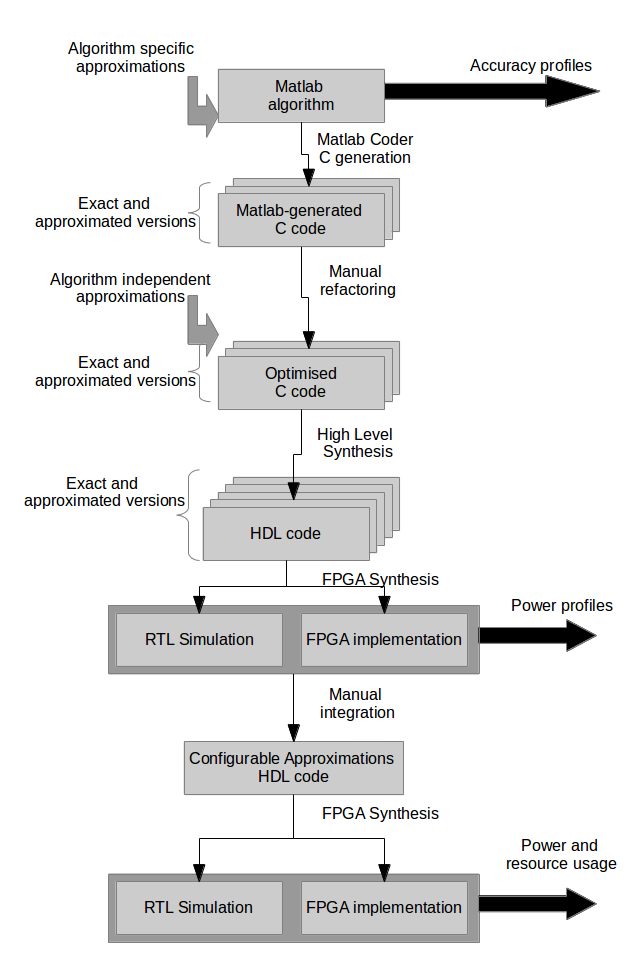
\includegraphics[width=0.9\columnwidth]{img/experimental_flow.png}
  \caption{Experimental design flow.}
  \label{fig:experimental_flow}
\end{figure}


\subsection{Dynamic approximations using prior knowledge}
The results of dynamically performing the approximation using the algorithms explained in Section \ref{learning} and \ref{sec:EKF} are detailed here. First, using the approximation results of each individual step, an "approximation level" is defined. To do this, various combinations of the micro approximations are sorted in ascending order according to their accuracy error. This results in a vector of tuples containing pairs of indexes (used as the approximation level) and strings indicating the approximation combination. 

The first tuple in this vector corresponds to the approximation method, which generates the highest accuracy. Its last element, however, creates the weakest accuracy.
At each filtering step, in order to use different approximation combinations, the approximation level is either increased or decreased. Determining whether to increment or decrement the approximation level is performed by evaluating the KL divergence result (\ref{eq:KLDIV2}).

\begin{figure}[tb]
  \centering
  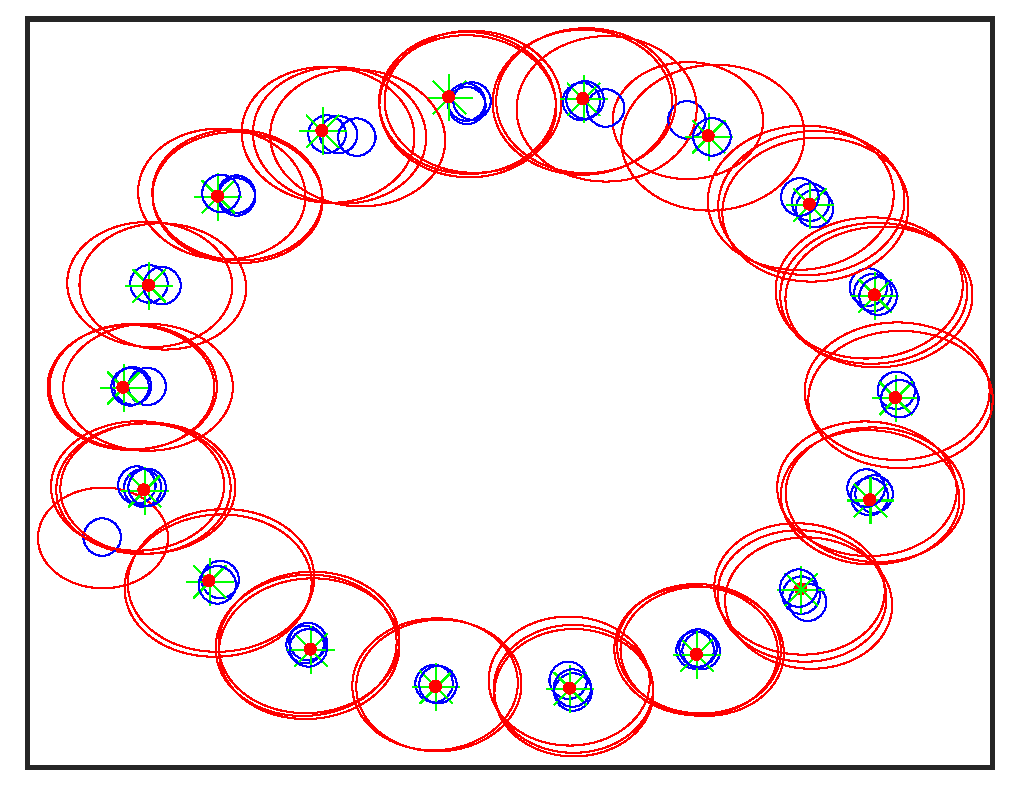
\includegraphics[width=0.9\columnwidth]{img/Tracks_plot_cropped.eps}
  \caption{Every 100 iteration overlay plot of the tracks and true states for an overall 5000 iterations.}
  \label{fig:track_res}
\end{figure}

The result of the overlay tracking plot using dynamic approximation in various iterations is shown in Fig.~\ref{fig:track_res} for a total number of iterations 5000. 
The red ellipses represent the covariance matrix ${\bf \Sigma}_{X,k}$ (\ref{eq:correctCOV}) at every iteration, the blue circles show $[x_k, y_k]^\intercal$ and green asterisks with red dots are the locations of true states $[\bar{x}_k, \bar{y}_k]^\intercal$. 

At every iteration, KL divergence is computed according to (\ref{eq:KLDIV2}), with sample stack size $N = 75$.  If it is less than a given threshold $T$ (for our results in Fig. \ref{fig:track_res}, $T = 0.5$) the approximation level is incremented. Otherwise, it is decremented to have a more precision tracking performance. The Euclidean distance between the found track and true state is computed for each iteration and shown in Fig.~\ref{fig:KL_and_err}-a, as well as the KL divergence in Fig.~\ref{fig:KL_and_err}-b. When the KL divergence goes above $T$ in Fig.~\ref{fig:KL_and_err}, the accuracy deteriorates. The approximation level is then immediately reduced in order to compensate the accuracy. Therefore, in only a few more iterations the accuracy again increases. This causes median accuracy error of 0.1661 (m) with median KL divergence 1.2098 for 5000 iterations.

\begin{figure}
    \centering
    \begin{subfigure}[tb]{0.5\textwidth}
        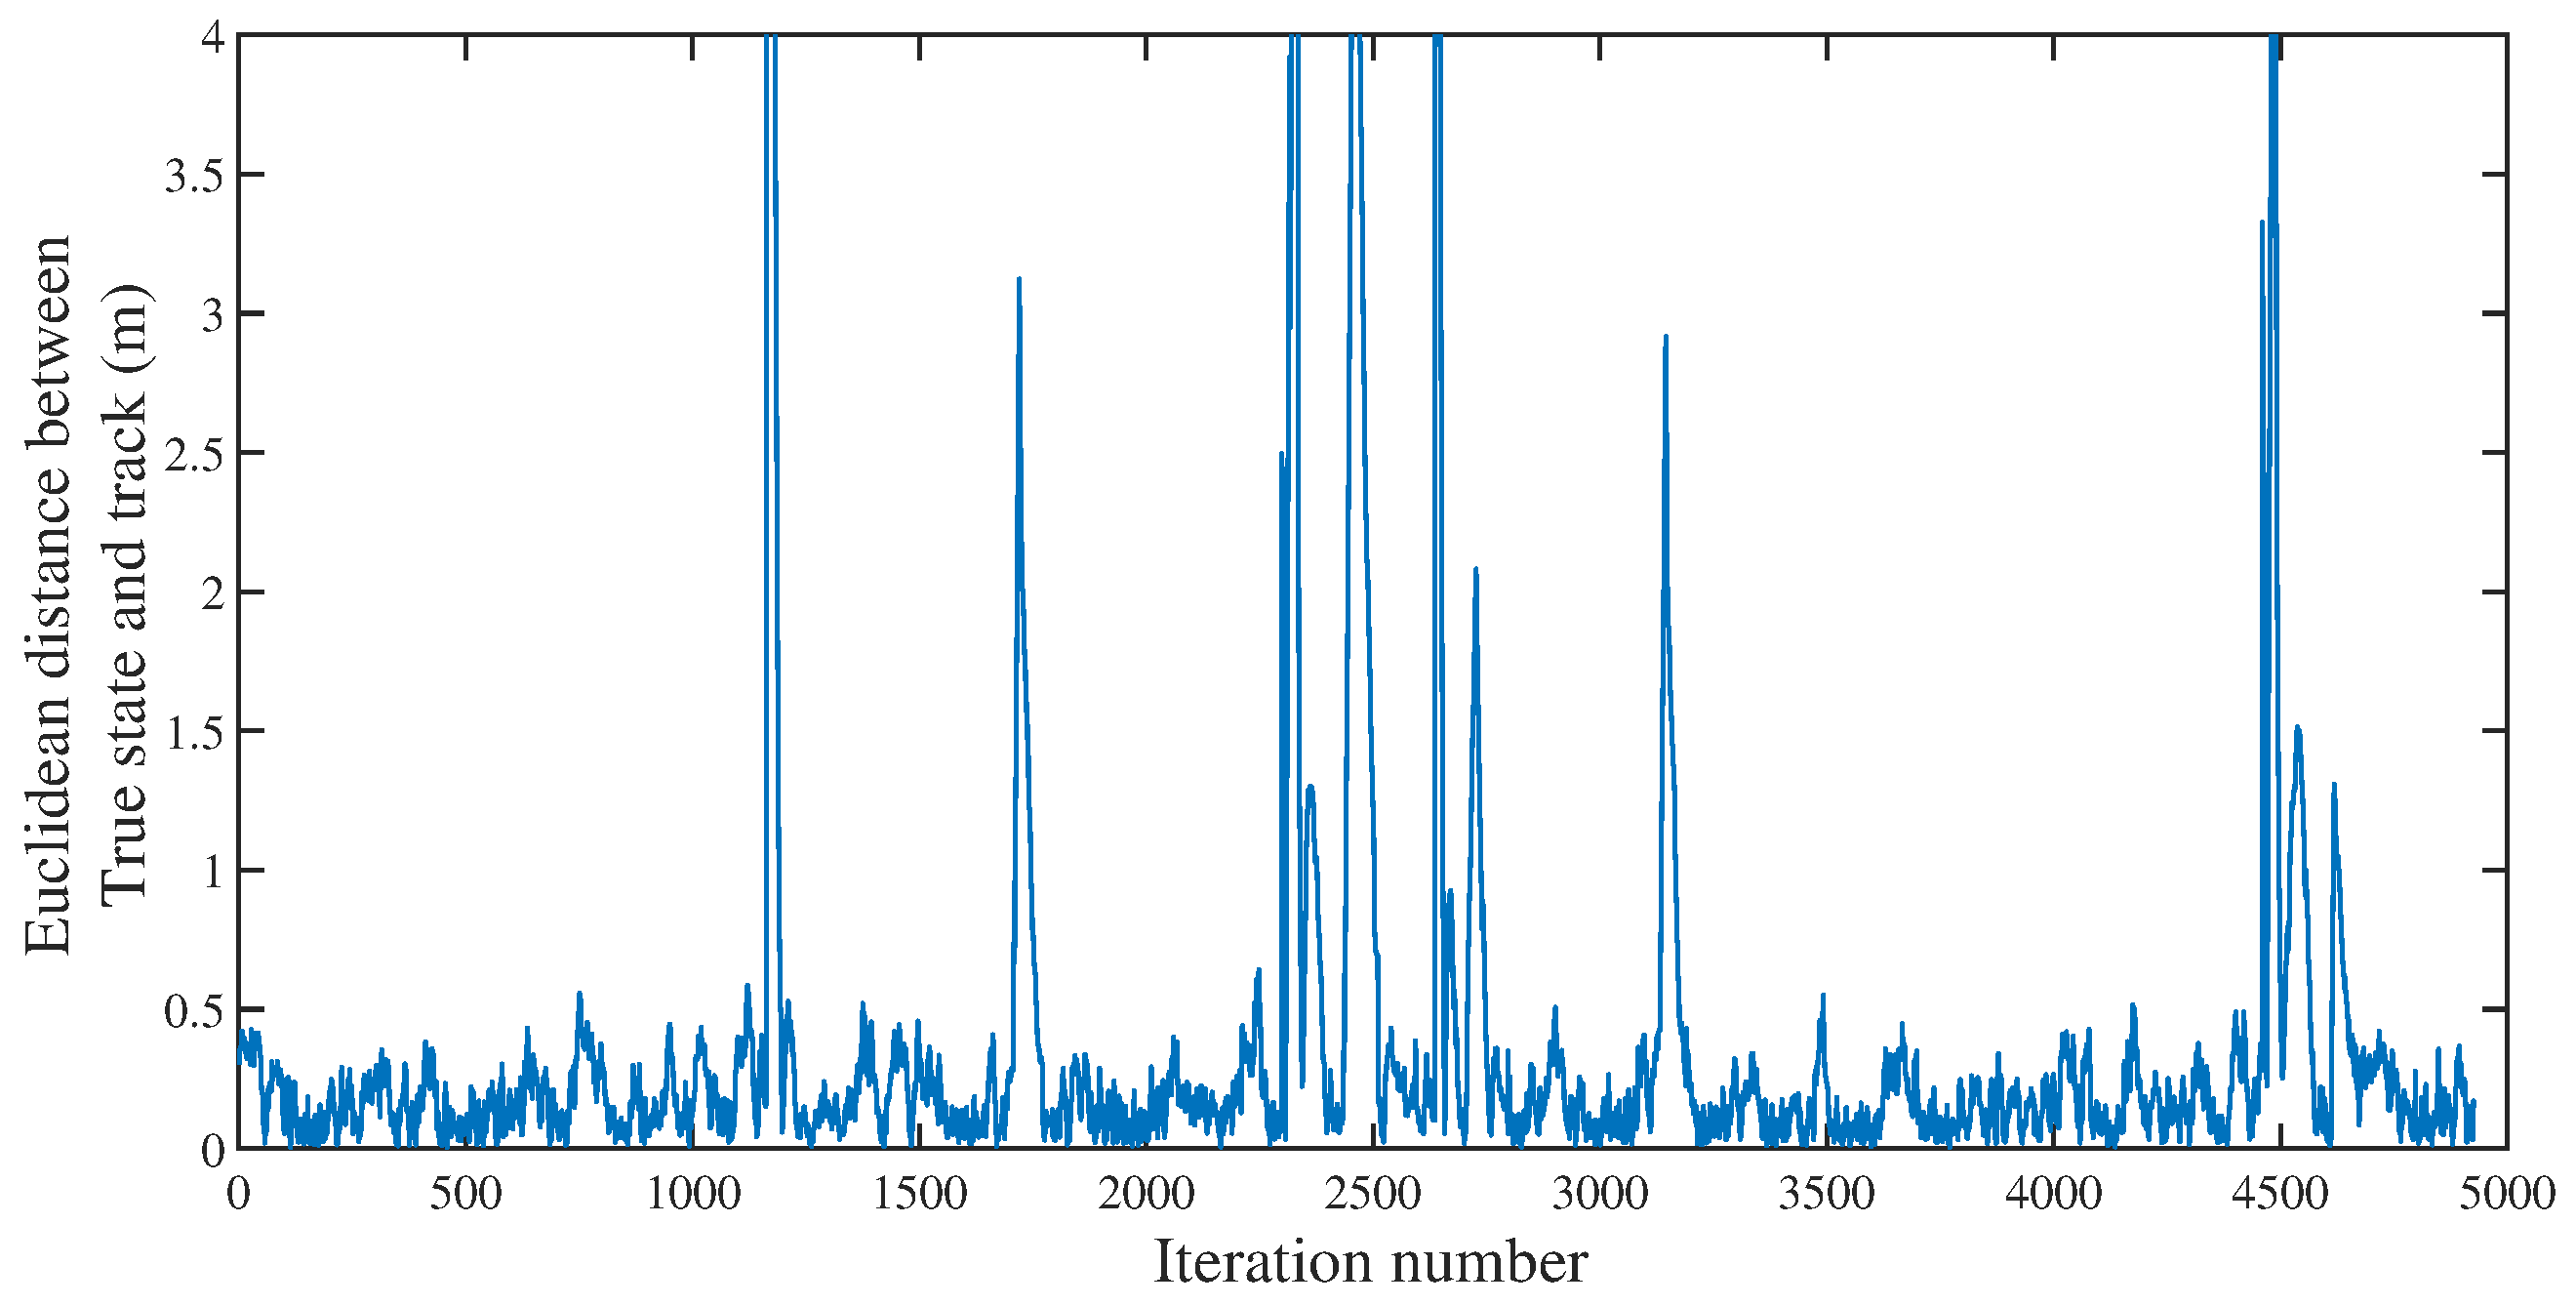
\includegraphics[width=\textwidth]{img/Err_figure_cropped.eps}
        \caption{}
        \label{fig:gull}
    \end{subfigure}
    \begin{subfigure}[tb]{0.5\textwidth}
        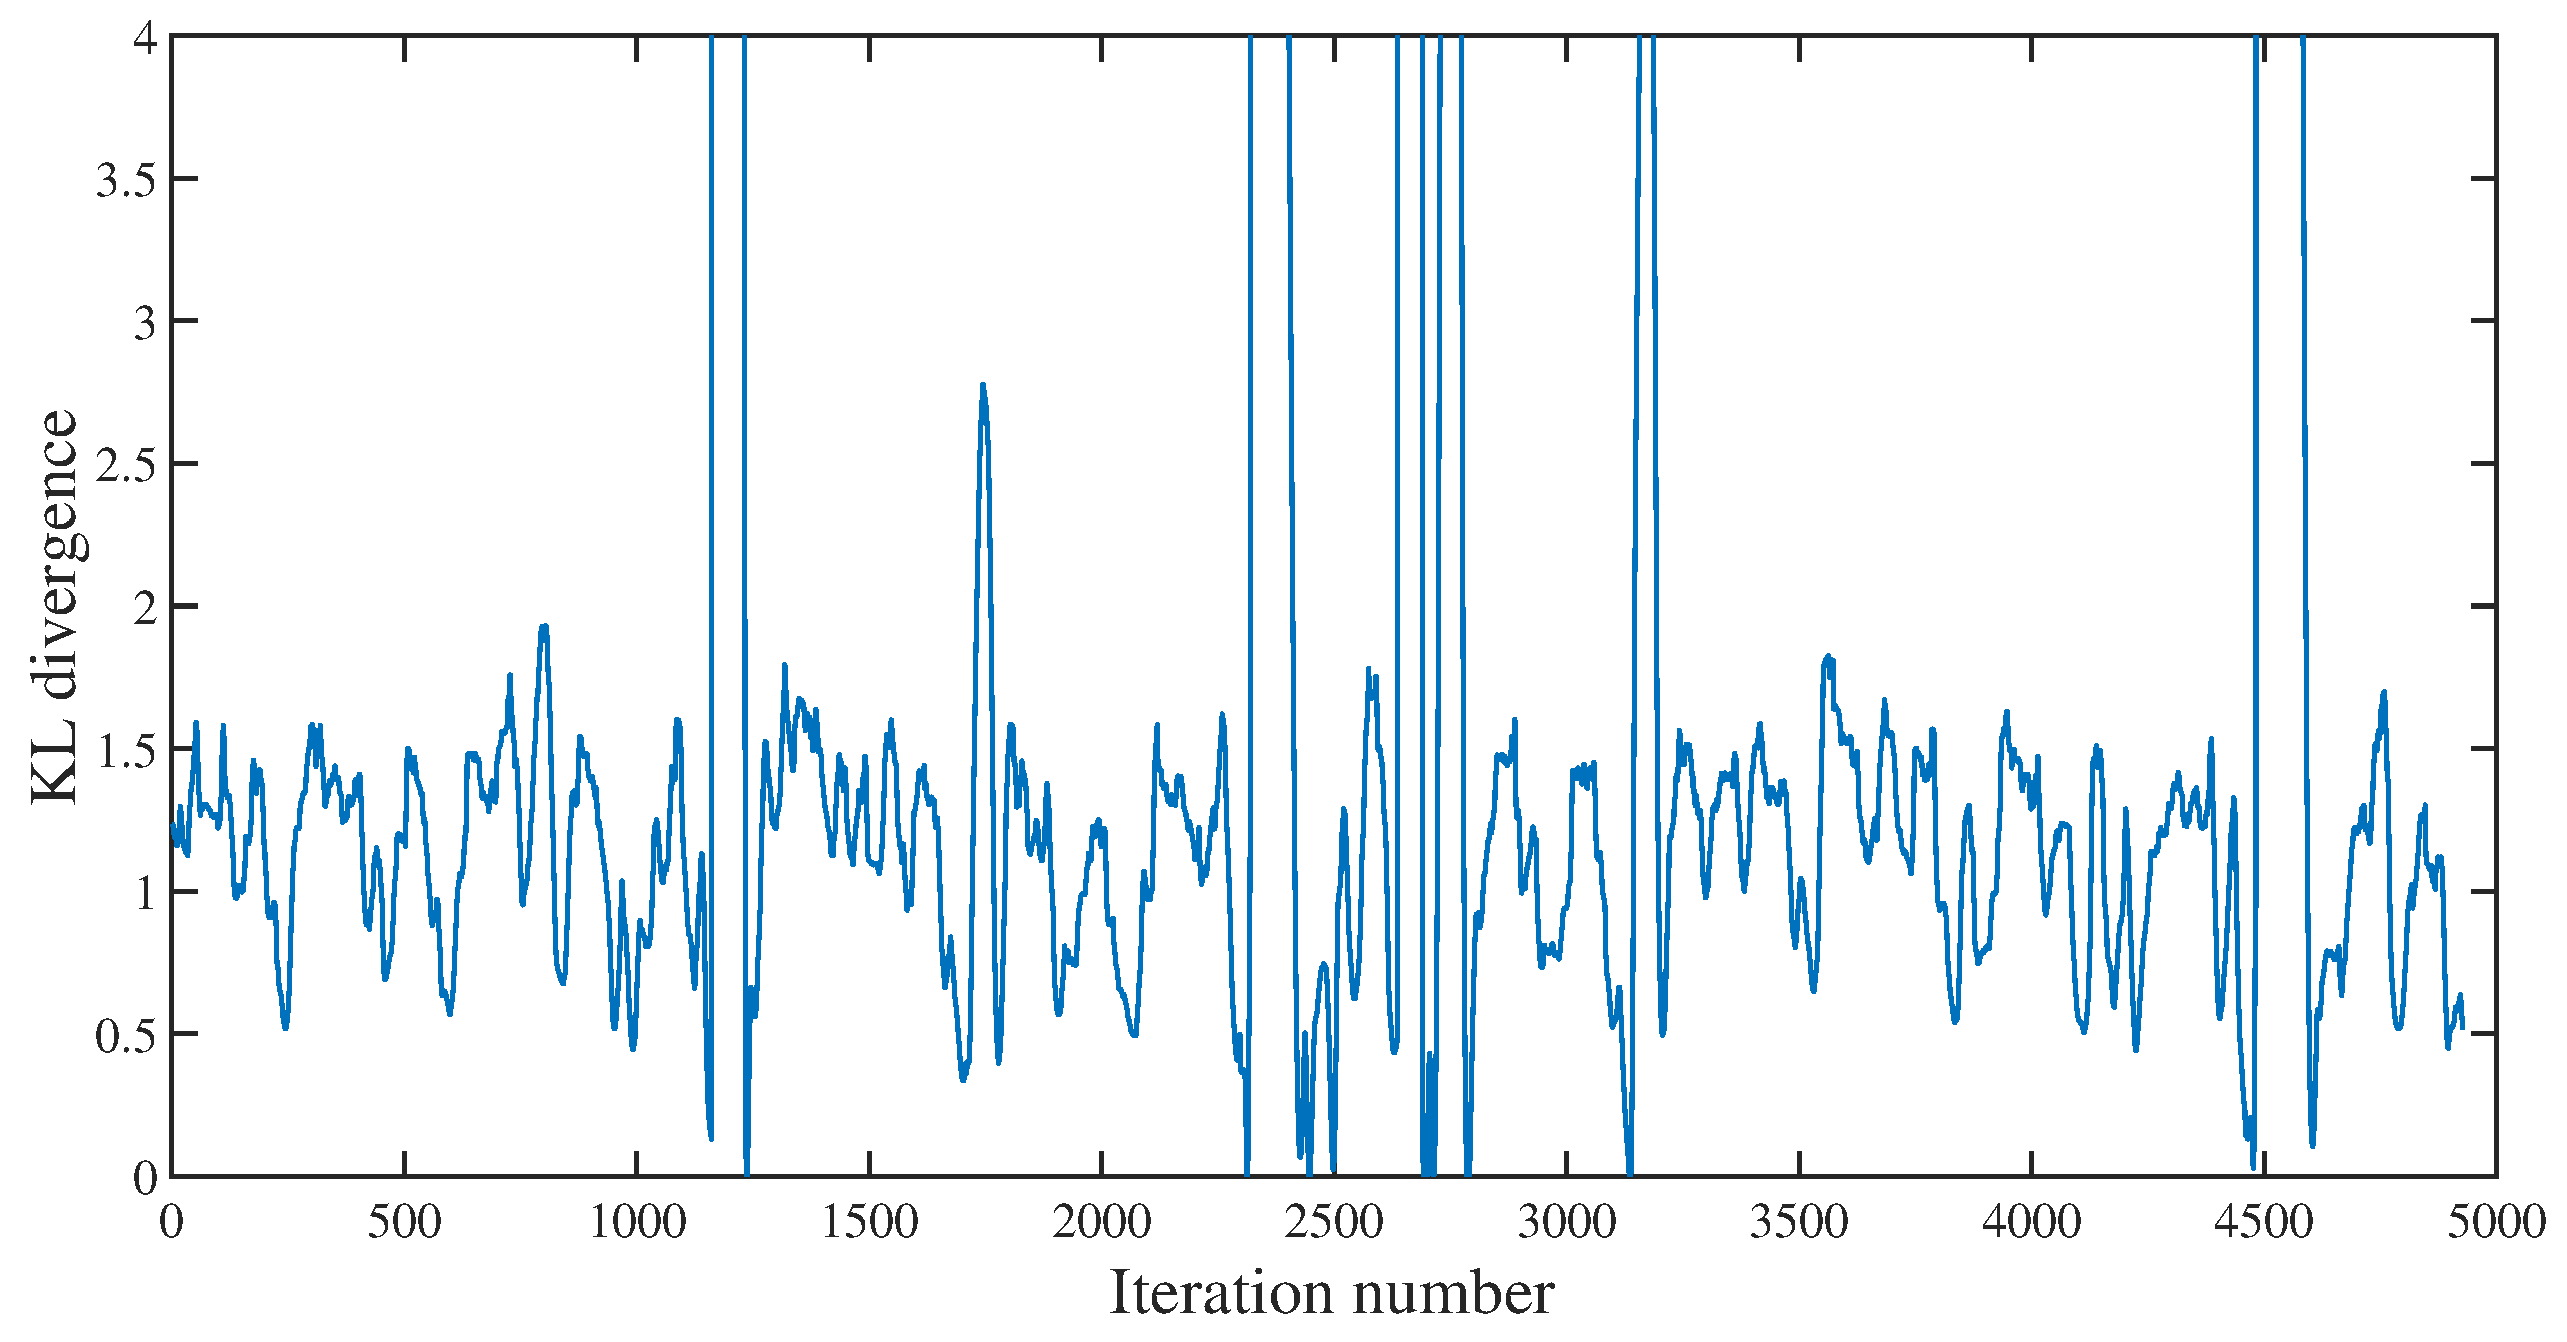
\includegraphics[width=\textwidth]{img/KL_figure_cropped.eps}
        \caption{}
        \label{fig:tiger}
    \end{subfigure}
    \caption{(a) Euclidean distance between the true state and tracks; (b) Corresponding KL divergence.}
    \label{fig:KL_and_err}
\end{figure}

Using the power profiles in Table \ref{table:power_profiles_comb}, the consumed energy of each approximation can be computed by multiplying the power with the time resolution ($\Delta t = 0.1$ (s)). The accumulated energy is plotted in Fig. \ref{fig:Energy_res_acc} for the last 1500 iterations. 
The baseline which consumes a constant power of 0.799 (W), results in a total of $\approx 394$ (J). However, the accumulated energy consumption for the dynamic approximation case is $\approx 384$ (J). This shows about $2.54 \%$ energy reduction.
By compromising over the accuracy result and increasing the KL divergence threshold, more intense approximations can be obtained, which results in even lower energy consumption. This is shown in Fig.~\ref{fig:Energy_res_acc} as the dashed green and cyan lines for thresholds 1.5 and 4.0, respectively

\begin{figure}[tb]
  \centering
  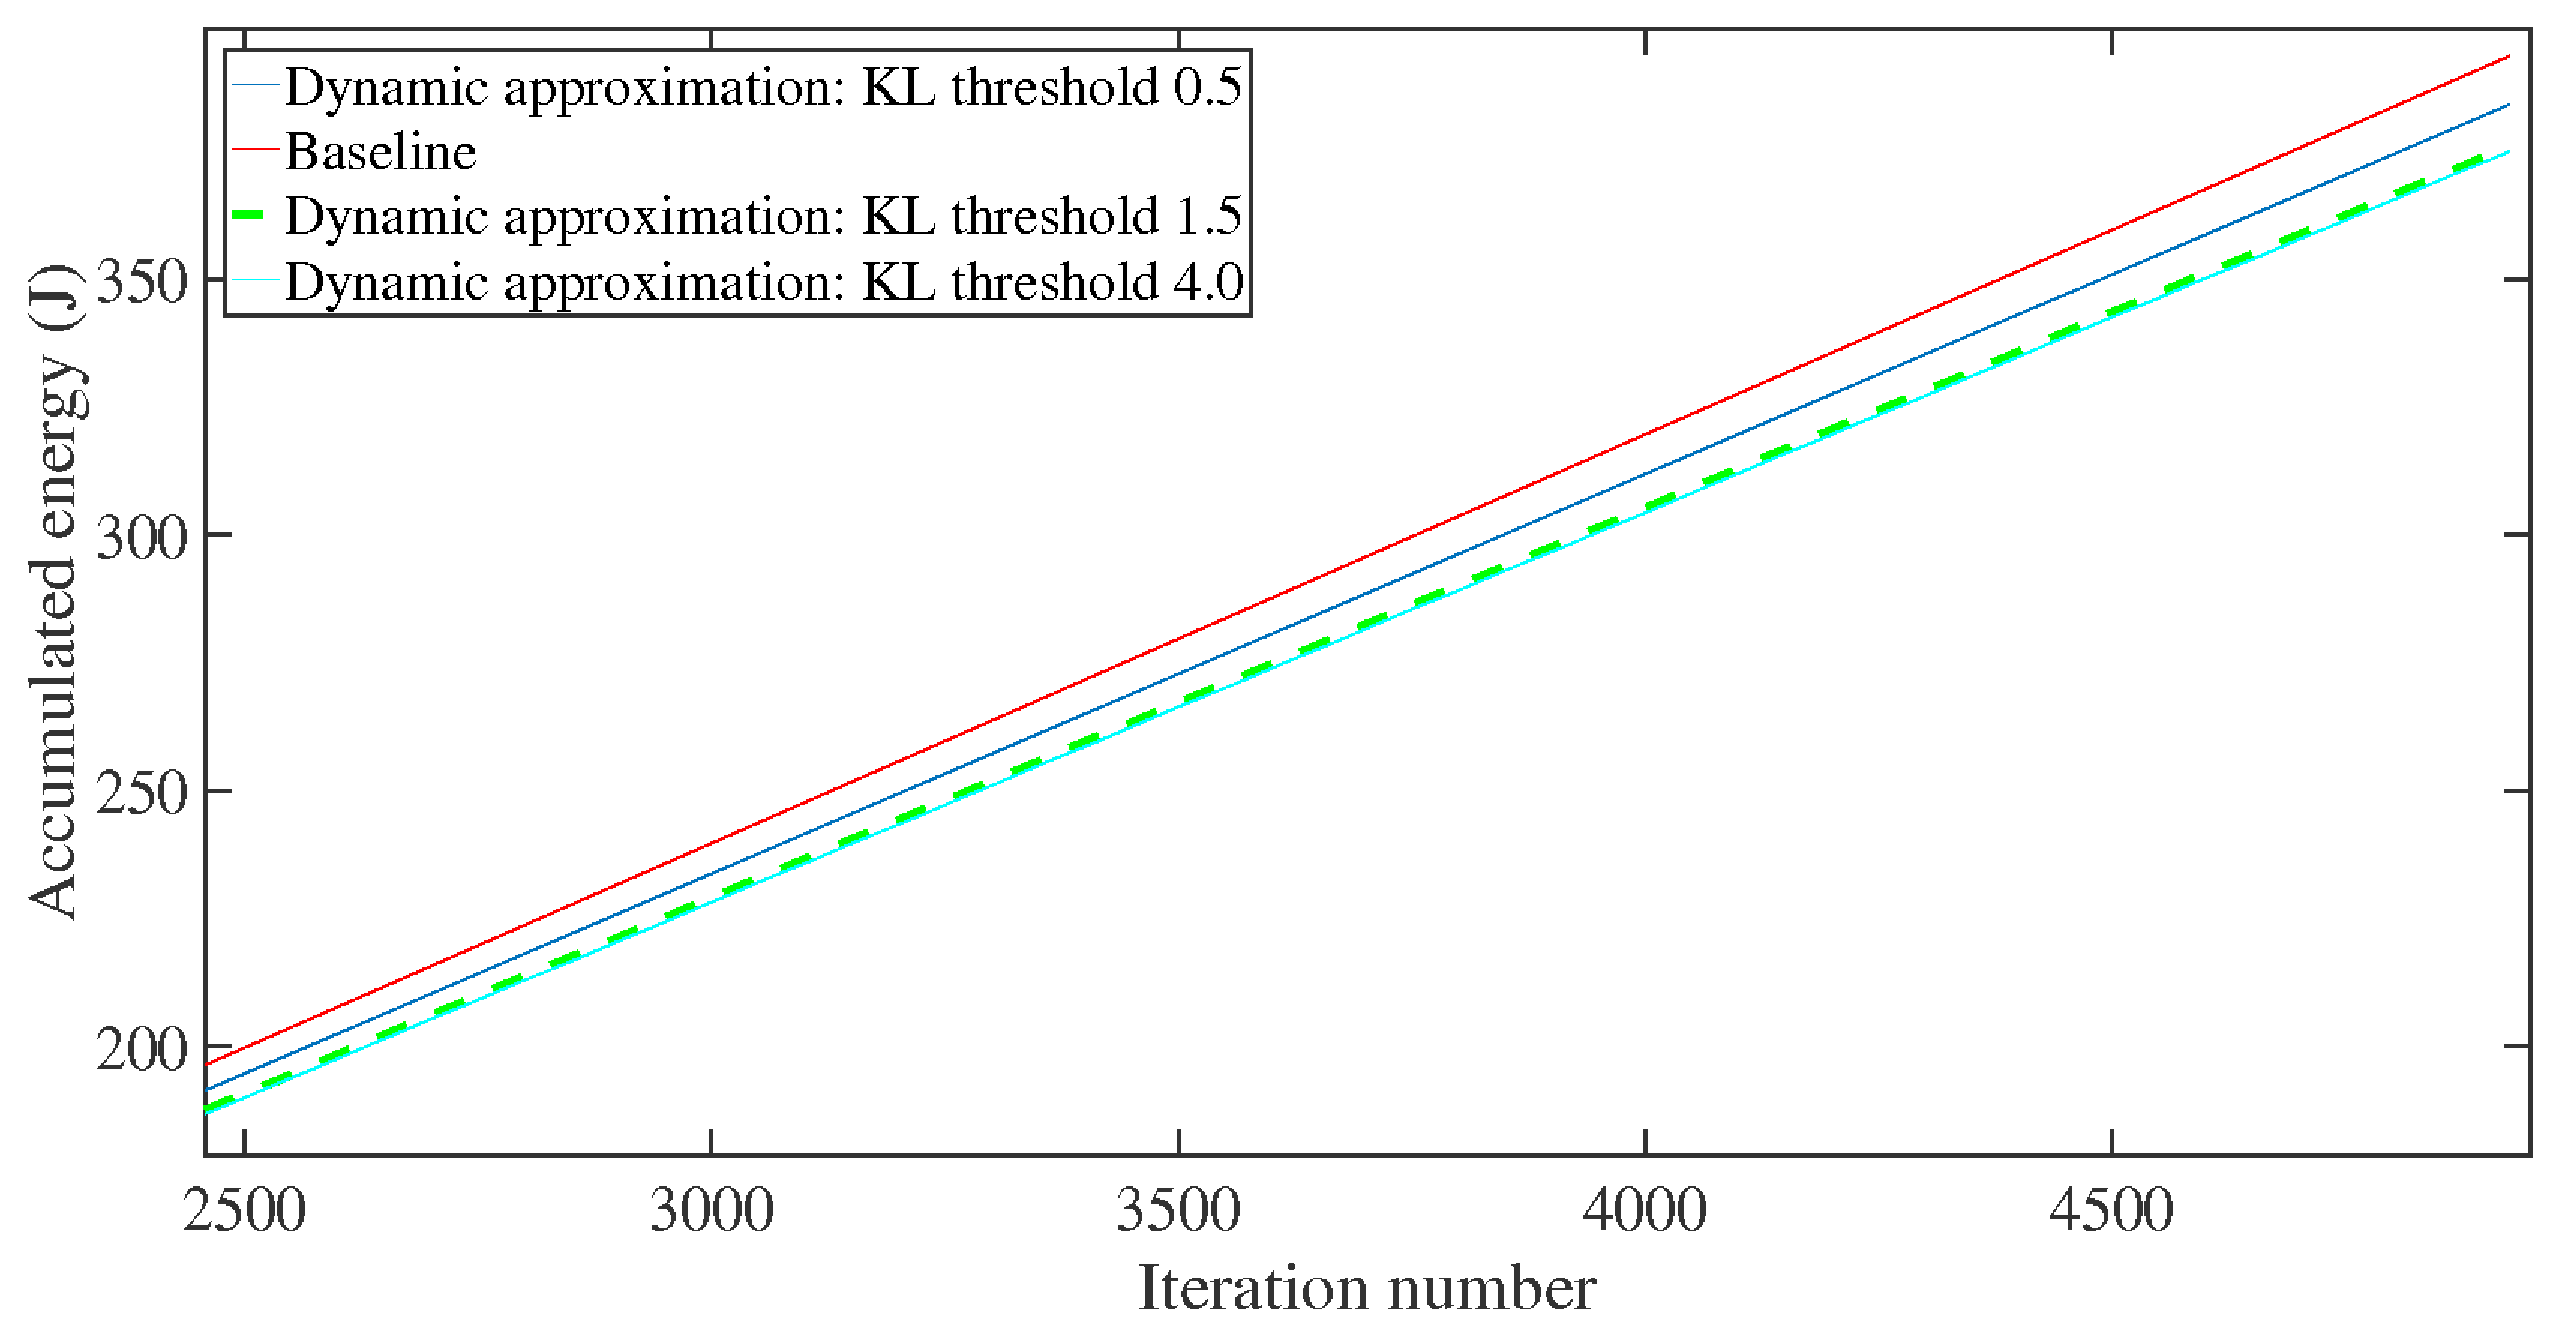
\includegraphics[width=1\columnwidth]{img/Energy_cropped.eps}
  \caption{Accumulated energy consumption for the baseline (no approximation) and dynamic approximations, with three different KL divergence thresholds.}
  \label{fig:Energy_res_acc}
\end{figure}